\documentclass[11pt,a4paper,oneside]{article}
\usepackage[T1]{fontenc} 
\usepackage[utf8]{inputenc}
\usepackage[main=english]{babel}
\usepackage{graphicx}                       % 1pt = 0.035146cm
\usepackage{float}
\graphicspath{{Figures/}}
\usepackage[justification=default]{subfig}  % Manage sub-figures 
\usepackage[update]{epstopdf}
\usepackage[labelfont=bf]{caption}
\usepackage{titlesec}                       % Allows customization of titles
\usepackage{booktabs}
\usepackage{color}
\usepackage[textwidth = 450pt,top = 80pt, bottom = 60pt]{geometry}
\usepackage{threeparttable}
\usepackage{soul}
\newcommand{\hlc}[2][yellow]{{\sethlcolor{#1}\hl{#2}}}
\usepackage[inline]{enumitem}
\usepackage[symbol]{footmisc}

\renewcommand{\thefootnote}{\fnsymbol{footnote}}

%--------------------------------------------------------------------------------
%       MATH PACKAGES
%--------------------------------------------------------------------------------
\usepackage{amsmath}
%\usepackage{mathtools}
\usepackage[leqno,fleqn,intlimits]{empheq}
\usepackage{bm}
%\usepackage{amssymb}
\usepackage{empheq}
\usepackage[inline]{enumitem}
%--------------------------------------------------------------------------------
%       MATLAB CODE
%--------------------------------------------------------------------------------
\usepackage{mcode}
%--------------------------------------------------------------------------------
%       MY COMMANDS
%--------------------------------------------------------------------------------
\renewcommand{\vec}[1]{\mathbf{#1}}
\newcommand{\tr}{\textcolor{red}}
\newcommand{\mathbi}[1]{\bm{\textbf{\em #1}}}
%--------------------------------------------------------------------------------
%       BIBLIOGRAPHY PACKAGES
%--------------------------------------------------------------------------------
% \usepackage{csquotes}
% \usepackage[sorting=nyt,%
% sortcites=true,%
% bibencoding=ascii,%
% autopunct=true,%
% hyperref=true,%
% language=auto,%
% %backref=true,%
% url=false,%
% maxcitenames=10,%
% minbibnames = 3,%
% maxbibnames=3,%
% giveninits, 
% natbib = false,
% isbn=false,%
% backend=biber]{biblatex}
% \addbibresource{bibliograhy_assignment.tex}
%--------------------------------------------------------------------------------
%       MISCELLANEA
%--------------------------------------------------------------------------------
\usepackage[]{hyperref}
\usepackage{cleveref}
%%% CREF setup
\crefname{equation}{Eq.}{Eqs.}
\crefname{table}{Table}{Tables}
\crefname{figure}{Fig.}{Figs.}
\setlength{\parindent}{0pt}

%--------------------------------------------------------------------------------
%       TITLE SECTION
%--------------------------------------------------------------------------------
\newcommand\headlinecolor{\normalcolor}

\makeatletter
\renewcommand*\maketitle{
    \begingroup
    \centering
    \fontsize{14.4}{14.4}       % 72pt on 80pt leading
    \selectfont
    \headlinecolor
    \@title\\
    \vspace{5mm}
    \@author
    \par
    \vskip1in
    \endgroup
    \vspace{-22mm}
}
\makeatother

\title{MSAS -- Assignment \#2: Simulation}  % Article title
\author{\large Matteo Baio, 232805}
\date{}

%--------------------------------------------------------------------------------
% HEADING packages
\usepackage{fancyhdr}   % Headers and footers control
\setlength{\headheight}{32pt}
\pagestyle{fancyplain}  % Defines a new header for all pages (absolutely all pages, use fancy to exclude title-page and chapters, if book class is used) 
\fancyhf{}              % clears the header and footer, otherwise the elements of the default "plain" page style will appear
\lhead{Matteo Baio, MSAS -- Assignment \#2}
\rhead{\vspace{-0.5cm}\includegraphics[width=0.3\textwidth]{newlogo.eps}}
\lfoot{AY 2023-24 -- Prof.\ F.\ Topputo; TA: C.\ Balossi, S.\ Borgia}
\rfoot{\thepage}

%--------------------------------------------------------------------------------
%       BEGIN DOCUMENT
%--------------------------------------------------------------------------------
\begin{document}
\maketitle
\thispagestyle{fancy}

%--------------------------------------------------------------------------------
%       MODELING PARADIGMS, BASIC SYSTEMS
%--------------------------------------------------------------------------------
\section{Exercise 1}
The rocket engine in Figure \ref{fig:therm} is fired in laboratory conditions.
With reference to Figure \ref{fig:therm}, the nozzle is made up of an inner lining ($k_1$), an inner layer having specific heat $c_2$ and high conductivity $k_2$, an insulating layer having specific heat $c_4$ and low conductivity $k_4$, and an outer coating ($k_5$).
The interface between the conductor and the insulator layers has thermal conductivity $k_3$.

\subsection*{1.1) Part 1: Parameters definition}
Select the materials of which the nozzle is made of\footnote{The interface layer is not made of a physically existing material, though it produces a thermal resistance.
For this layer, the value of the thermal resistance $R_3$ can be direcly assumed, so avoiding to choose $k_3$ and $\ell_3$.}, and therefore determine the values of $k_i$ ($i=1,\dots,5$), $c_2$, and $c_4$.
Assign also the values of $\ell_i$ (i=1,\dots,5), $L$, and $A$ in Figure \ref{fig:therm}.
\begin{figure}[ht!]
    \centering
    \includegraphics[width=0.8\textwidth]{Figures/fig_therm.pdf}
    \caption{\label{fig:therm} Real thermal system.}
\end{figure}

\subsection*{1.2) Part 2: Causal modeling}
Derive a physical model and the associated mathematical model using one node per each of the five layers and considering that only the conductor and insulator layers have thermal capacitance.
The inner wall temperature, $T_i$, as well as the outer wall temperature, $T_o$, are assigned.
Using the mathematical model, carry out a dynamic simulation \underline{in MATLAB} to show the temperature profiles across the different sections.
At initial time, $T_i(t_0)=T_o(t) = 20\ {\rm C^\circ}$. When the rocket is fired, $T_i(t) = 1000\ {\rm C^\circ}$, $t\in[t_1,\,t_f]$, following a ramp profile in $[t_0,\,t_1]$.
Integrate the system using $t_1 = 1\ {\rm s}$ and $t_f = 60\ {\rm s}$.

\subsection*{1.3) Part 3: Acausal modeling}
a) Reproduce \underline{in Simscape} the physical model derived in Part 2. Run the simulation from $t_0 = 0\ {\rm s}$ to $t_f = 60\ {\rm s}$ and show the temperature profiles across the different sections. Compare the results with the ones obtained in point 1.2). 
b) Which solver would you choose? Justify the selection based on the knowledge acquired from the first part of the course.
c) Repeat the simulation in Simscape implementing two nodes for the conductor and insulator layers and show the temperature profiles across the different sections.
\medskip

\medskip \hrule \medskip
\rightline{\small(15 points)}
\medskip

The nozzle materials are defined following approximately the available data of the SpaceX Raptor engine and reported \cref{tab:ex1_material}.
The cross section area $A$ and the length $L$ of the nozzle are fixed and respectively equal to $4\,m^2$ and $1\,m$.
\begin{table}[H]
    \centering
    \begin{threeparttable}
    \caption{\label{tab:ex1_material} Nozzle materials and properties}
        \begin{tabular}{llcccc}
            \toprule
            \toprule
            Layer           & Material              & $l_i, m$  & $\rho, \frac{kg}{m^3}$    & $c_{pi}, \frac{J}{kgK}$   & $k_i, \frac{W}{mK}$  \\ 
            \midrule
            Inner lining    & $Inconel$             & $0.02$    & $8840$                    & $--$                      & $14.5$ \\ 
            Conductor       & $Copper$              & $0.03$    & $8960$                    & $385$                     & $400$ \\ 
            Interface\tnote{$\star$} &              & $0.01$    & $--$                      & $--$                      & $--$ \\ 
            Insulator       & $Ceramic$             & $0.02$    & $2800$                    & $800$                     & $1.5$ \\     
            Outer coating   & $Stainless\,steel$    & $0.02$    & $8000$                    & $--$                      & $16$ \\ 
            \bottomrule
            \bottomrule
        \end{tabular}
        \begin{tablenotes}
            \footnotesize
            \item[$\star$] Thermal resistance value fixed $K=0.000678\,K/W$
        \end{tablenotes}
    \end{threeparttable}
\end{table}

Once defined all the nozzle dimensions and materials, the thermal resistance and capacitance are computed following \cref{eq:ex1_thermalR} and \cref{eq:ex1_thermalC}.
\begin{empheq}[]{align}
    R_i &= \frac{l_i}{k_i\,A}   \label{eq:ex1_thermalR} \\
    C_i &= \rho_i A l_i c_{pi}  \label{eq:ex1_thermalC}
\end{empheq}

The different nozzle layers are modelled following the electric circuit analogy. 
A physical model of the system is derived considering one node for each of the five layers as represented in \cref{fig:ex1_phyModelCase1}.
\begin{figure}[H]
    \centering
    \includegraphics[width=1\textwidth]{Figures/ex1_phyModelCase1.pdf}
    \caption[]{\label{fig:ex1_phyModelCase1} Physical model with one node for each layer}
\end{figure}

The model can be simplified by computing the equivalent resistance between the different nodes; the math is reported in \cref{eq:ex1_eqResistence}.
\begin{subequations}
    \begin{align}
        R_{i2} &= R_1 + \frac{R_2}{2}                   \label{eq:ex1_Ri2} \\
        R_{24} &= \frac{R_2}{2} + R_3 + \frac{R_4}{2}   \label{eq:ex1_R24} \\
        R_{4o} &= \frac{R_4}{2} + R_5                   \label{eq:ex1_R4o}
    \end{align}
    \label{eq:ex1_eqResistence}
\end{subequations}

Note that only conductor and insulator layers have thermal capacitance as suggested from the exercise instruction.
This assumption simplifies quite a lot the mathematical formulation since, in absence of capacitance, the heat flow can be assumed constant.
As consequence the \cref{eq:ex1_heatFlow} can be written.
\begin{equation}
    \begin{cases}
        Q_{i1} = Q_{i2} = Q_{12} \\
        Q_{23} = Q_{24} = Q_{34} \\
        Q_{45} = Q_{4o} = Q_{5o} 
    \end{cases}
    \label{eq:ex1_heatFlow}
\end{equation}

All the heat flows can be easily put in relationship with the nodes temperature value by means of \cref{eq:ex1_heatVsTemp}.
\begin{equation}
    Q_{i2} = \frac{T_i-T_2}{R_{i2}}  \qquad Q_{24} = \frac{T_2-T_4}{R_{24}}  \qquad Q_{4o} = \frac{T_4-T_o}{R_{4o}}
    \label{eq:ex1_heatVsTemp}
\end{equation}

The temperature evolution in time of nodes $T_2$ and $T_4$ is obtained solving numerically the ODEs \cref{eq:ex1_T2} and \cref{eq:ex1_T4}. 
\begin{empheq}[]{align}
    \dot{T_2} &= \frac{Q_{i2}-Q_{24}}{C_2}    \label{eq:ex1_T2} \\
    \dot{T_4} &= \frac{Q_{24}-Q_{4o}}{C_4}    \label{eq:ex1_T4}
\end{empheq}

Finally even $T_1$, $T_3$ and $T_5$ nodes temperature can be evaluated over time by exploiting the heat flows relationship previously written (\cref{eq:ex1_heatFlow} and \cref{eq:ex1_heatVsTemp}) as done in \cref{eq:ex1_T1}, \cref{eq:ex1_T3} and \cref{eq:ex1_T5}.
\begin{empheq}[]{align}
    T_1 &= T_i - Q_{i2} \frac{R_1}{2}       \label{eq:ex1_T1} \\
    T_3 &= T_4 + Q_{24} \frac{R_3+R_4}{2}   \label{eq:ex1_T3} \\
    T_5 &= T_o + Q_{4o} \frac{R_5}{2}       \label{eq:ex1_T5}
\end{empheq}

The IVP obtained combining \cref{eq:ex1_T2} and \cref{eq:ex1_T4} can be integrated in MATLAB using different algorithms.
To understand which is the best method to use an eigenvalues analysis is performed to find out if the system analysed has some particular characteristics.

Firstly the \cref{eq:ex1_T2} and \cref{eq:ex1_T4} are rewritten in matrix form considering $\vec{T}=[T_2;T_4]$ as presented in \cref{eq:ex1_matrixForm}.
\begin{equation}
    \frac{d \vec{T}}{dt} = \vec{A} \vec{T} =    \left[
    \begin{array}{cc}
        -\left( \frac{1}{C_2 R_{i2}} + \frac{1}{C_2 R_{24}} \right) & \frac{1}{C_2 R_{24}} \\
        \frac{1}{C_4 R_{24}} & -\left( \frac{1}{C_4 R_{24}} + \frac{1}{C_4 R_{4o}} \right)
    \end{array}                                 \right] \vec{T}
    \label{eq:ex1_matrixForm}
\end{equation}

The eigenvalues of matrix $\vec{A}$ are shown in \cref{fig:ex1_eigenvalues} and results equal to $\lambda_1=-0.0086$ and $\lambda_2=-0.0045$.
\begin{figure}[H]
    \centering
    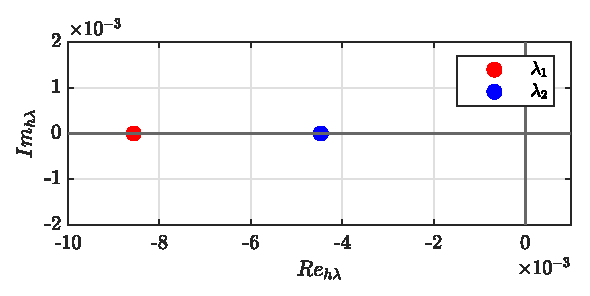
\includegraphics[width=0.45\textwidth, keepaspectratio]{Figures/ex1_eigenvalues.eps}
    \caption[]{\label{fig:ex1_eigenvalues} System eigenvalues}
\end{figure}

The problem turns out to be stable and only marginally stiff.
The second eigenvalue results about half of the first one, with both presenting the same order of magnitude.
From this analysis can be concluded that a nonstiff method such as \mcode{ode45} might be suitable for integration.
Another good candidate might also be \mcode{ode23t}, which is ideal for solving only moderately stiff problems.

The choice of \mcode{ode45} is also confirmed by the automatic ODE selector built-in in MATLAB.

The thermal problem is also solved in Simscape by building the physical model shown in \cref{fig:ex1_simscapeCase1}.
\begin{figure}[htb]
    \centering
    \includegraphics*[width=1\textwidth, keepaspectratio]{Figures/ex1_simscapeCase1.pdf}
    \caption[]{\label{fig:ex1_simscapeCase1} Simscape model with one node for each layer}
\end{figure}

To solve the problem Simscape builds a DAEs system to compute simultaneously all the nodes temperature.
By doing so methods that guarantees efficiency in solving Differential-algebraic system of equations, as \mcode{daessc} or \mcode{ode23t}, are suggested. 

In \cref{fig:ex1_tempNodes} the temperature profiles of the different nodes obtained on MATLAB with \mcode{ode45} and \mcode{ode23t} are reported and compared with the one obtained on Simscape using \mcode{ode23t}.
\begin{figure}[H]
    \centering
    \includegraphics*[width=0.7\textwidth, keepaspectratio]{Figures/ex1_tempKeyNodes.eps}
\end{figure}
\begin{figure}[H]
    \centering
    \includegraphics*[width=0.8\textwidth, keepaspectratio]{Figures/ex1_tempOtherNodes.eps}
    \caption[]{\label{fig:ex1_tempNodes} Temperature nodes evolution over time}
\end{figure}

Both in MATLAB and Simscape the maximum step size has been manually set to $h=0.01$.
Note that the temperature curves obtained with the different methods are perfectly overlapped.
The same conclusion can be made observing \cref{fig:ex1_tempCompare} where all the nodes temperature are plotted on the same graph.
On the left the temperature obtained integrating the problem on MATLAB with \mcode{ode45} is shown, while on the right the results obtained on Simscape with \mcode{ode23t} are reported.
\begin{figure}[H]
    \centering
    \includegraphics*[width=0.8\textwidth, keepaspectratio]{Figures/ex1_tempCompare.eps}
    \caption[]{\label{fig:ex1_tempCompare} System temperature profile with MATLAB and Simscape}
\end{figure}

Note that \mcode{ode23t} is picked, instead of \mcode{daessc}, for the Simscape simulation because of the important differences of the temperature evolution trends over time.

An analysis on the time cost of the different methods has also been performed.
For each method a cycle of 50 runs is executed, the time needed to complete these tasks is measured and post processed by means of an arithmetic mean.
In this phase a bigger pool of integration method is considered, this allows to verify if the considerations previously done, based on the eigenanalysis results, are correct.
The integration methods tested on MATLAB are \mcode{ode45}, \mcode{ode89}, \mcode{ode113}, \mcode{ode23t} and \mcode{ode15s}, while the Simscape simulation is, once again, done with \mcode{ode23t}.
The results of the analysis are reported in the histogram shown in \cref{fig:ex1_CPUtime}.
\begin{figure}[H]
    \centering
    \includegraphics*[width=0.5\textwidth, keepaspectratio]{Figures/ex1_CPUtime.eps}
    \caption[]{\label{fig:ex1_CPUtime} CPU-time cost histogram}
\end{figure}

As expected \mcode{ode45} turns out to be the best method to integrate the thermal problem on MATLAB.
\mcode{ode23t} applied on MATLAB model performs a little bit worse than expected, probably due to the fact that the problem isn't sufficiently stiff, while it works well on Simscape to solve the DAE system.

The temperature curves obtained through MATLAB \mcode{ode45} and \mcode{ode89} are then compared with the Simscape results.
This analysis is done to check if the bigger computational cost is justified by a higher precision.
To do so a time grid of 30 elements is built and the temperature value in each point is retrieved by means of a linear interpolation.
The results are shown in \cref{fig:ex1_errorCompare}.
\begin{figure}[H]
    \centering
    \includegraphics*[width=0.75\textwidth, keepaspectratio]{Figures/ex1_errorCompare.eps}
    \caption[]{\label{fig:ex1_errorCompare} MATLAB integration error compared to Simscape}
\end{figure}

Both methods, as expected, present a very small error over all the time interval but, unfortunately, \mcode{ode89} doesn't perform clearly better than \mcode{ode45}.

Finally a more precise analysis is performed modifying the simscape model.
The number of nodes for conductor and insulator layers are increased to two and the mass of these two layers is considered located in two points, respectively at $1/4$ and $3/4$ of $l_i$ (\cref{fig:phyModelCase2} and \cref{fig:ex1_simscapeCase2}).
\begin{figure}[H]
    \centering
    \includegraphics*[width=1\textwidth, keepaspectratio]{Figures/ex1_phyModelCase2.pdf}
    \caption[]{\label{fig:phyModelCase2} Physical model with two nodes for conductor and insulator}
\end{figure}

\begin{figure}[H]
    \centering
    \includegraphics*[width=1\textwidth, keepaspectratio]{Figures/ex1_simscapeCase2.pdf}
    \caption[]{\label{fig:ex1_simscapeCase2} Simscape model with two nodes for conductor and insulator}
\end{figure}

Using, once again, \mcode{ode23t} as integration method and $h=0.01$ as maximum step size the new model nodes temperature are obtained and reported in \cref{fig:ex1_tempCase2}.
\begin{figure}[H]
    \centering
    \includegraphics*[width=0.6\textwidth, keepaspectratio]{Figures/ex1_tempCase2.eps}
    \caption[]{\label{fig:ex1_tempCase2} System temperature profile for \cref{fig:ex1_simscapeCase2} model}
\end{figure}


%--------------------------------------------------------------------------------
\clearpage
\section{Exercise 2}
The real system of an electric propeller engine is depicted in Figure \ref{fig:propeller}.
It is composed by a DC permanent magnet motor which drives a propeller shaft.
Between the motor and propeller shaft there is a single stage gear box to regulate the angular speed ratio.
Moreover, to avoid overheating of the gear unit, the system is augmented by a cooling system where a fluid exchanges heat with the gear box itself.
In Figure \ref{fig:blocks scheme} a functional breakdown structure of the system is shown. 

\begin{figure}[ht!]
    \centering
    \includegraphics[width=0.8\textwidth]{Figures/RealSystem_msas.png}
    \caption{\label{fig:propeller} Real system.}
\end{figure}

\begin{figure}[ht!]
    \centering
    \includegraphics[width=0.9\textwidth]{Figures/BlockScheme_msas.png}
    \caption{\label{fig:blocks scheme} Functional block scheme of the system.}
\end{figure}

\subsection*{2.1) Part 1: Propeller Electric Engine}
Considering the real system in \ref{fig:propeller} \textbf{without} the cooling part, you are asked to:
\begin{enumerate}
    \item Extract a physical model highlighting assumptions and simplifications.    
    \item Reproduce the model in acausal manner in Dymola.
    \item According to the block scheme in \ref{fig:blocks scheme}, tune a controller (e.g., a PID controller) such that the motor input voltage remains less than 200 V and the error signal \textbf{Err} is less than 0.1 rad/s after 10 s. 
    \item Study the Gear box temperature and heat flux for a simulation time of $\mathbf{t_f}$ = 120 s (considering only conduction as heat transfer).
    \item Discuss the simulation results and the integration scheme used
\end{enumerate}

For the simulation part, you shall consider: the DC motor data listed in Table \ref{tab:dc}; the gear box data listed in Table \ref{tab:gear}, with loss parameters in Table \ref{tab:gear2}; a propeller made of \textbf{aluminium} with nominal angular speed $\hat{\omega}$ and a nominal quadratic speed load torque $\hat{T}_{load}$ acting on it (Table \ref{tab:prop}).
The reference angular speed signal to be tracked by the propeller is given in Figure \ref{fig:refsignal}. 

\begin{table}[ht!]
    \centering
    \caption{DC motor data}
    \begin{tabular}{ |c|c|c| } 
        \hline
        \textbf{Parameter} & \textbf{Value} & \textbf{Unit}\\
        \hline
        Coil Resistance & 0.1 & $\Omega$  \\ 
        Inductance & 0.01 & H  \\ 
        Motor Inertia & 0.001 & kg $m^2$  \\ 
        Motor Constant & 0.3 & Nm/A \\ 
        \hline
    \end{tabular}
    \label{tab:dc}
\end{table}

\begin{table}[ht!]
    \centering
    \caption{Gear Box data}
    \begin{tabular}{ |c|c|c| } 
        \hline
        \textbf{Parameter} & \textbf{Value} & \textbf{Unit}\\
        \hline
        Mass & 3 & kg  \\ 
        Gear ratio & 2 & [-]  \\ 
        Specific heat & 1000 & J/(kg K)   \\ 
        Thermal Conductivity & 100 & Wm/K \\ 
        \hline
    \end{tabular}
    \label{tab:gear}
\end{table}
        
\begin{table}[ht!]
    \centering
    \caption{Gear Box Loss Table}
    \begin{tabular}{ |c|c|c| } 
        \hline
        \textbf{Driver angular speed [rad/s]} & \textbf{Mesh efficiency[-]} & \textbf{Bearing friction torque [Nm]}\\
        \hline
        0 & 0.99 & 0  \\ 
        50 & 0.98 & 0.5  \\ 
        100 & 0.97 & 1  \\ 
        210 & 0.96 & 1.5  \\ 
        \hline
    \end{tabular}
    \label{tab:gear2}
\end{table}

\begin{table}[ht!]
    \centering
    \caption{Propeller data}
    \begin{tabular}{ |c|c|c| } 
        \hline
        \textbf{Parameter} & \textbf{Value} & \textbf{Unit}\\
        \hline
        Diameter & 0.8 & m  \\ 
        Thickness & 0.01 & m  \\ 
        $\hat{\omega}$ & 210 & rad/s \\
        $\hat{T}_{load}$ & 100 & Nm \\
        \hline
    \end{tabular}
    \label{tab:prop}
\end{table}

\begin{figure}[ht!]
    \centering
    \includegraphics[width=0.8\textwidth]{Figures/ReferenceSignal.png}
    \caption{\label{fig:refsignal} Angular speed reference for the propeller.}
\end{figure}

\subsection*{2.2) Part 2: Cooling System}
After the previous gear unit thermal analysis, now consider the steady-state condition reached by the propeller engine at the end of the simulation to model and simulate a single \textbf{fixed} volume flow rate cooling system (as shown in Figure \ref{fig:propeller}) for the gear unit and considering only \textbf{convection} as heat transfer. In particular, you are asked to:

\begin{enumerate}
    \item Derive a physical model highlighting assumptions and simplifications.
    \item Reproduce the acausal model in Dymola.
    \item Tune the cooling system in terms of volume flow rate, control logics, and initial fluid storage temperature such that:
    \begin{enumerate}
        \item the gear unit is kept between 40$^{\circ}$C and 60$^{\circ}$C.
        \item the source tank does not get empty before the end simulation time
        \item the storage tanks have a maximum height of 0.8 $m$ and cross section area of 0.01 $m^2$
        \item the system shall have a recirculating capability in order to exploit the outlet fluid for a next cooling process (when the source tank get empty)
        \item the sink heated fluid is kept between 5$^{\circ}$C and 10$^{\circ}$C.
        \item the power consumption of the thermal system shall be no more than 6 kW 
    \end{enumerate}
    \item Discuss the simulation results and the integration scheme used
\end{enumerate}

For the simulation part consider properties of water at 10$^{\circ}$C as cooling incompressible fluid (convective thermal conductance $\lambda_{conv}$ = 300 W/K) and the cylindrical pipe line data listed in Table \ref{tab:pipe}.
The simulation shall last at least $\mathbf{t_{sim}}$ = 300 s starting with no water along the pipe.

\begin{table}[ht!]
    \centering
    \caption{Pipe line properties}
    \begin{tabular}{ |c|c|c| } 
        \hline
        \textbf{Parameter} & \textbf{Value} & \textbf{Unit}\\
        \hline
        Diameter & 4 & cm  \\ 
        Length & 40 & cm  \\ 
        Geodetic height & 0 & m \\
        Friction losses & 0 & [-] \\ 
        \hline
    \end{tabular}
    \label{tab:pipe}
\end{table}

\medskip
\medskip \hrule \medskip
\rightline{\small(15 points)}
\clearpage

Starting from the real system a physical model is retrieved by means of some assumption and simplification on its components. 

The DC motor is modelled as a circuit composed by a voltage source, a fixed resistor, a fixed inductor and a rotor with its inertia.
Both the inductor resistance and resistor inductance are considered negligible.
The voltage source receives as input a signal which is then translated in voltage while the rotor converts the voltage signal in rotational mechanical energy.

The gearbox is modelled as a ''lossy gear'', a built-in block in modelica, connected to a thermal conductivity and capacitance block.
All the data, including the loss table, is given as user input to these blocks to correctly model the gearbox behaviour.

The propeller is considered rigid and its inertia is modelled as a rod with the pole positioned in its centre.

The physical system has no delay between input and the state, uncertainty and noise are neglected and all input data are considered constant in time. 
The just presented model, built following a lumping approach, is shown in \cref{fig:ex2a_droneModel}.
\begin{figure}[H]
    \centering
    \includegraphics*[width=1\textwidth, keepaspectratio]{Figures/ex2a_blockDiag.pdf}
    \caption[]{\label{fig:ex2a_droneModel} Dymola physical model of the propeller electric engine}
\end{figure}

The integration scheme picked for the simulation is \mcode{dassl}, but also \mcode{lsodar} and \mcode{rk4fix} are tested.
The choice is made after a comparison between these three methods.
In \cref{tab:ex2a_compInteg} the main data concerning the performance of each method are reported.
\begin{table}[H]
    \centering
    \caption{Compare between different integration schemes for \cref{fig:ex2a_droneModel} system}
    \label{tab:ex2a_compInteg}
    \begin{tabular}{lcccc}
        \toprule
        \toprule
            Method          & CPU-time integration  & CPU-time grid interval    & Feval & Max order \\ 
        \midrule
            \mcode{dassl}   & 0.002 $sec$           & 0.004 $millisec$          & 360   & 5         \\
            \mcode{lsodar}  & 0.006 $sec$           & 0.012 $millisec$          & 368   & 5         \\
            \mcode{rk4fix}  & 0.005 $sec$           & 0.010 $millisec$          & 2000  & 4         \\
        \bottomrule
        \bottomrule
    \end{tabular}
\end{table}

In the considered system the input signal to the voltage source is regulated by a PID controller manually tuned to match the system requirements (given in the exercise instruction).
The obtained tuning of the PID is reported in \cref{tab:ex2a_tuningPID}.
\begin{table}[H]
    \centering
    \caption{PID tuning values}
    \label{tab:ex2a_tuningPID}
    \begin{tabular}{ccc}
        \toprule
        \toprule
            Gain - $k$  & Integrator - $T_i$  & Derivative - $T_d$ \\ 
        \midrule
            0.085       & 0.185 $sec$         & 0.5 $sec$  \\
        \bottomrule
        \bottomrule
    \end{tabular}
\end{table}

The motor input voltage and the difference between the reference angular velocity and the actual one (defined as $error$) are shown in \cref{fig:ex2a_voltage}, \cref{fig:ex2a_error} and \cref{fig:ex2a_errorZoom}.
Their envelop over time confirms that the voltage is always less than $200\,V$ and the $error$, apart from the first transitory, is always less than $0.1\,rad/s$.
\begin{figure}[H]
    \centering
    \includegraphics*[width=0.5\textwidth, keepaspectratio]{Figures/ex2a_voltage.pdf}
    \caption[]{\label{fig:ex2a_voltage} Motor input voltage}
\end{figure}
\begin{figure}[H]
    \centering
    \begin{minipage}{0.45\textwidth}
        \centering
        \includegraphics*[width=\textwidth, keepaspectratio]{Figures/ex2a_error.pdf}
        \caption[]{\label{fig:ex2a_error} PID Signal error}
    \end{minipage}
    \hspace{0.05\textwidth}
    \begin{minipage}{0.45\textwidth}
        \centering
        \includegraphics*[width=\textwidth, keepaspectratio]{Figures/ex2a_errorZoom.pdf}
        \caption[]{\label{fig:ex2a_errorZoom} Zoom of \cref{fig:ex2a_error}}
    \end{minipage}
\end{figure}

The gear box is the only component of the physical system that heats up, for this reason its thermal proprieties are analysed more in depth.   
The heat flux, after a small transitory, reaches a constant value of $Q=2210.9\,W$ as reported in \cref{fig:ex2a_gearHeat}, while the temperature, as expected, linearly increases over time.
After $120s$, as shown in \cref{fig:ex2a_gearTemp}, the temperature reaches $T=103.295\,^{\circ}C$.
\begin{figure}[H]
    \centering
    \begin{minipage}{0.45\textwidth}
        \centering
        \includegraphics*[width=\textwidth, keepaspectratio]{Figures/ex2a_gearHeat.pdf}
        \caption[]{\label{fig:ex2a_gearHeat} Gear box wall heat flux}
    \end{minipage}
    \hspace{0.05\textwidth}
    \begin{minipage}{0.45\textwidth}
        \centering
        \includegraphics*[width=\textwidth, keepaspectratio]{Figures/ex2a_gearTemp.pdf}
        \caption[]{\label{fig:ex2a_gearTemp} Gear box wall temperature}
    \end{minipage}
\end{figure}

From this analysis is clear that a cooling system is needed, otherwise the temperature would increase indefinitely leading to component failure.
A physical model of such a system is retrieved from the real one considering some assumptions and created in Dymola as shows \cref{fig:ex2b_coolingModel}.
\begin{figure}[H]
    \centering
    \includegraphics*[width=0.9\textwidth, keepaspectratio]{Figures/ex2b_blockDiag.pdf}
    \caption[]{\label{fig:ex2b_coolingModel} Dymola physical model of the propeller electric engine}
\end{figure}

The gear box is the only heat source of the system and the convection with the water of the cooling system is the only form of heat exchange considered. 
As for the previous model, there is no delay between input and the state, uncertainty and noise are neglected and all input data are considered constant in time. 

Considering the cooling loop must be point out that no friction effects in the pipe line are modelled and the volume flow doesn't present any transient.
The whole system is also considered isolated, no mass or heat exchange is considered with the environment around it.

The source and storage tanks present the same dimensions and the recirculation is considered guaranteed once the storage tank temperature is kept under control.

To match the requirements on gearbox wall and cooling fluid temperature two control logics based on ''hysteresis'' and ''boolean'' blocks are added to the system.
The gearbox temperature is kept between $40\,^{\circ}C$ and $60\,^{\circ}C$ thanks to a controller which regulates the volume flow of the medium in the pipe line.
The volume flow rate is regulated based on the output of a sensor which measures the gear wall temperature in every time instants.
The results of the tuned system obtained during the simulation are shown in \cref{fig:ex2b_gearWallTemp}, \cref{fig:ex2b_sourceTankFlow} and \cref{fig:ex2b_sourceTankLevel}.
\begin{figure}[H]
    \centering
    \includegraphics*[width=0.5\textwidth, keepaspectratio]{Figures/ex2b_gearWallTemp.pdf}
    \caption[]{\label{fig:ex2b_gearWallTemp} Gear box wall temperature with cooling system}
\end{figure}
\begin{figure}[H]
    \centering
    \begin{minipage}{0.45\textwidth}
        \centering
        \includegraphics*[width=\textwidth, keepaspectratio]{Figures/ex2b_sourceTankFlow.pdf}
        \caption[]{\label{fig:ex2b_sourceTankFlow} Source tank volume flow}
    \end{minipage}
    \hspace{0.05\textwidth}
    \begin{minipage}{0.45\textwidth}
        \centering
        \includegraphics*[width=\textwidth, keepaspectratio]{Figures/ex2b_sourceTankLevel.pdf}
        \caption[]{\label{fig:ex2b_sourceTankLevel} Source tank water level}
    \end{minipage}
\end{figure}

In a similar way a simple thermal system is implemented to regulate the temperature of the fluid in the storage tank.
As defined in the requirements, the system is tuned to avoid that the power consumption exceeds the limit value of $6\,kW$.
Once again the obtained results are shown in \cref{fig:ex2b_storageTankCooling} and \cref{fig:ex2b_storageTankTemp}.
\begin{figure}[H]
    \centering
    \begin{minipage}{0.45\textwidth}
        \centering
        \includegraphics*[width=\textwidth, keepaspectratio]{Figures/ex2b_storageTankCooling.pdf}
        \caption[]{\label{fig:ex2b_storageTankCooling} Storage tank heat flow}
    \end{minipage}
    \hspace{0.05\textwidth}
    \begin{minipage}{0.45\textwidth}
        \centering
        \includegraphics*[width=\textwidth, keepaspectratio]{Figures/ex2b_storageTankTemp.pdf}
        \caption[]{\label{fig:ex2b_storageTankTemp} Storage tank temperature}
    \end{minipage}
\end{figure}

The integration scheme used to obtain the reported results is \mcode{dassl}.
Anyway, as done before, some simulations with other methods are executed to find out if better integration scheme can be used.
In \cref{tab:ex2b_compInteg} the main performance values of \mcode{dassl}, \mcode{lsodar} and \mcode{rk4fix} are reported.
\begin{table}[H]
    \centering
    \caption{Compare between different integration scheme for \cref{fig:ex2b_coolingModel} system}
    \label{tab:ex2b_compInteg}
    \begin{tabular}{lcccc}
        \toprule
        \toprule
            Method          & CPU-time integration  & CPU-time grid interval    & Feval & Max order \\ 
        \midrule
            \mcode{dassl}   & 0.003 $sec$           & 0.006 $millisec$          & 445   & 3         \\
            \mcode{lsodar}  & 0.001 $sec$           & 0.002 $millisec$          & 178   & 4         \\
            \mcode{rk4fix}  & 0.001 $sec$           & 0.002 $millisec$          & 2000  & 4         \\
        \bottomrule
        \bottomrule
    \end{tabular}
\end{table}

\clearpage
\end{document}

%--------------------------------------------------------------------------------
%       END DOCUMENT
%--------------------------------------------------------------------------------